\documentclass[]{aastex6}

\usepackage{amsmath}
\usepackage{graphicx,epstopdf}
\usepackage{natbib}
%\usepackage[left=1in]{geometry}
\bibliographystyle{apj}


\DeclareMathOperator{\sech}{sech}



% Common Math Operators Defined by Jake

\newcommand{\curl}{\nabla \times}
\newcommand{\grad}{\nabla}
\newcommand{\pardiv}[3]{\frac{\partial^{#3} {#1}}{\partial {#2}^{#3}}}
\newcommand{\adiv}[1]{\frac{D {#1}}{Dt}}
\newcommand{\adivlong}[1]{\frac{\partial{#1}}{\partial t} + (\mathbf{u} \cdot \nabla){#1}}


\begin{document}
\title{Bursts, Bombs, and Explosive Events: Magnetic Reconnection in the Lower Solar Atmosphere} 

\author{Jacob D. Parker}
\affil{Department of Physics, Montana State University,
  Bozeman, Montana 59717}

%\keywords{cool keyword}

%\linenumbers



\begin{abstract}
	Write an abstract.

%\date{Draft: \today}
\end{abstract}

\section{Background}
%This section needs to be 1) Compelling and 2) Convey a Depth of Understanding

	\begin{figure}
		\label{fig:reconnect}
		\caption{Here we present a cartoon representing an ideal presentation of magnetic reconnection and corresponding spectral observation.  Panel a shows Petscheck reconnection with bi-directional outflow jets at the Alfv\'en Speed, $v_a$.  Plotted along side is a theoretical line profile, for the labeled \textit{Line Of Sight} (LOS), showing two seperate peaks in intensity at $\pm v_a$. Panel b shows the developement of magnetic islands during the onset of the tearing mode instability.  The addition of stationary emitting material will fill out line center and result in a broadened, mostly centered line profile. The blue, green, red coloring of the line profiles demonstrated how line intensity is binned in Figure \ref{fig:eecolor}.}
		
		\centerline{\input{reconnection_cartoon.pdf_tex}} 
		
	\end{figure}  
	\subsection{Transient Brightenings in the Lower Solar Atmosphere}
	
	%Likely going to need some citations in this section.
	
	From the photosphere to the upper reaches of the transition region the solar atmosphere changes three orders of magnitude in temperature over only a few thousand kilometers.  This thin layer of the Sun, while often less grand in appearance than the corona, plays an important role in the energy transport required to heat the corona to mega-Kelvin temperatures.  Like the flickering coals of a camp fire the photosphere, chromosphere, and transition region are littered with small, short lived, brightenings.  Brightenings give us clues as to how often, where, and when energy produced in the solar interior is deposited beyond the photosphere.
	
	These small brightenings are often accompanied by fast motion.  Spectroscopic observations reveal many events, over a range of heights and temperatures, that have Doppler velocities exceeding the local thermal speed.  In order for plasma velocities to exceed  thermal speeds there must be a conversion of a non-thermal energy source to kinetic energy. It is becoming widely accepted that this extra energy comes from the solar magnetic field.  Through magnetic reconnection the Sun's magnetic field eliminates high energy discontinuities and converts that energy in to the heating and motion of local plasma.  While repeated observations of non-thermal plasma motion within regions of complicated magnetic field has the solar physics community leaning toward magnetic reconnection as the cause of solar atmospheric heating the details are still the subject of much debate.	

	\subsection{Ellerman Bombs and Explosive Events}
	
	Two commonly observed events in the Sun's lower atmosphere are Ellerman Bombs (EBs) and Explosive Events (EEs). EBs \citep{Ellerman1917} are commonly observed as intense brightenings in the wings of H$\alpha$ $\lambda 6563 \AA $ are characterized by small spatial scales (arcsecond or smaller) and short life times (a few minutes). H$\alpha$ has a peak formation temperature of $\approx 10000$ K placing EBs very low in the solar atmosphere near the photosphere. EBs are observed in regions of opposing magnetic polarity and, until recently \citep{Nelson2017}, exclusively within active regions.  EBs are believed to be the result of magnetic reconnection as new flux emerges through the photosphere and reconnects with the preexisting photopsheric magnetic field.  High resolution instruments such as the Crisp Imaging Spectropolarimeter \citep[CHRISP;][]{CHRISP} on the Swedish Solar Telescope \citep[SST;][]{SST} and the Interface Region Imaging Spectrometer \citep[IRIS;][]{IRIS} have helped discover more details about EBs.  They often originate between granules deep in the photosphere, have an upward extending flow or ``jet", and demonstrate very fast variations (on second timescales) coupled with repeated eruptions \citep{Watanabe2011,Vissers2013,Vissers2015}
	
	
	EEs were first analyzed by \citet{Brueckner1983} using data from the High Resolution Telescope and Spectrograph (HRTS) sounding rocket. EEs are typically characterized by Doppler shifts on order $100$ km s$^{-1}$ and spatial scales of a few arcseconds \citep{Dere1989,Dere1994}.  Si {\sc IV} $\lambda 1393$\AA\ rasters taken by the Solar Ultraviolet Measurement of Emitted Radiation (SUMER) sounding rocket revealed an EE with bi-directional jets near small magnetic bi-poles on the solar surface \citep{Innes1997}.  This presentation was said to match the classic magneto-hydrodynamic (MHD) model of reconnection \citep{Petschek1964} quite well and is illustrated in Figure \ref{fig:reconnect}(a). Data from the first flight of the Multi-Order Solar EUV Spectrograph \citep[MOSES;][]{Fox2010} sounding rocket showed evidence of many explosive events in He II $\lambda$304\AA. While a large number of events showed clear bi-directional jets with Doppler velocities of approximately 100 km s$^{-1}$ \citep{Rust2017}, one event showed fast jets, offset spatially, with a bright stationary core \citep{Fox2010}.  \citet{Fox2010} identified a possible cause of the complicated spatial/spectral signature to be the Tearing Mode Instability \citep{Furth1963} as shown in Figure \ref{fig:reconnect}(b).
	
	\subsection{IRIS Bombs and UV Bursts}
	IRIS has been observing the transition region since late 2013.  In this short period of time several discoveries have been made that have challenged our understanding of reconnection in the lower solar atmosphere.  An early discovery by \citet{Peter2014} showed the presence of very cool, photospheric absorption lines in the wings of the Si IV $\lambda$1394\AA\ line. Transient brightenings in Si IV with these types of absorption features have been labeled ``IRIS Bombs'' or ``UV Bursts'' and are thought to be caused by magnetic reconnection. The presence of the Ni II and Fe II absorption lines, with peak formation temperatures of approximately 15,000K, implies that IRIS bombs actually occur in the photosphere.  Magnetic reconnection would heat plasma to at least 80,000K for Si IV formation, and emit through the cool photospheric plasma above it.
	
	IRIS has also observed many events most similar to traditional EEs.  While early work by \citet{Innes1997} showed EEs in Si IV to have bi-directional jets, later work by \citet{Innes2015} with IRIS Si IV data has shown EEs to have broad, almost triangular, line profiles with very bright cores and little to now sign of bi-directional flows.  This was originally attributed to the Tearing Mode instability based on MHD simulations and synthetic line profiles. This theory has been corroborated recently by the observation of very small ($\approx 0."2$) and fast (less than a second) brightenings by SST that are co-spatial with Si IV UV Burst spectra \citep{Rouppe2017}.  These small brightenings are taken to be direct observation of Tearing Mode islands at transition region scales.
	
	
	
	\subsection{Problem Statement} 
	Transient brightening in the lower solar atmosphere have many names and present themselves in a variety of ways. Names aside, these events have a lot in common.  Consistently we see energy releases with on order arcsecond spatial scales and second temporal scales. Spectrometers reveal that these small events have Doppler velocities exceeding local thermal speeds, and that they occur in a wide temperature band from $10^4$-$10^6$ K.  Due to their correlation with complex photospheric magnetic fields and super thermal velocities these events are all likely connected to magnetic reconnection. Advances in instrumentation and modeling reveal the structure of the photosphere, chromosphere, and transition region to very three dimensional.  This advancement in our understanding of the Sun's lower atmosphere allows us to ask and study some interesting questions:
	
		\begin{itemize}
	
			\item Are EEs, UV Bursts, EBs, and IRIS Bombs truly different events, or are they all small reconnection events happening in a variety of environments?
			\item If all of these events are associated with magnetic reconnection then what determines its presentation?
			\item What is the role of small reconnection events in transporting mass and energy to the corona?
			\item What can we learn about the role of the tearing mode instability in the onset of fast solar magnetic reconnection?
			
			
		\end{itemize}
	
	

\section{Technical Approach} 
%This section needs show that solving our problem is 3) Feasible and that our method is 4) robust to possible set backs.


\begin{figure}
	\label{fig:eemap}
	\caption{Example explosive event map from our software package}
	\centerline{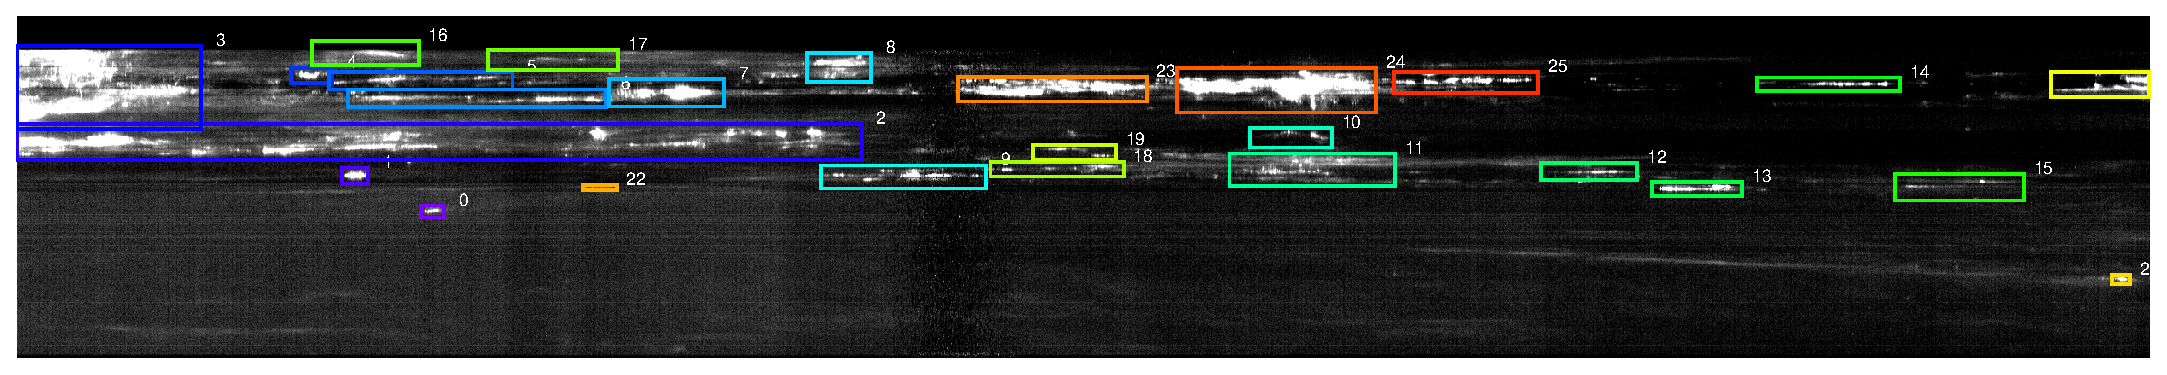
\includegraphics[scale=.5]{./NESSF_img/ee_map.eps}}
	
\end{figure}

\begin{figure}
	
	\caption{Event number 24 at a point in its evolution with a particularly sheared line profile.}
	\centerline{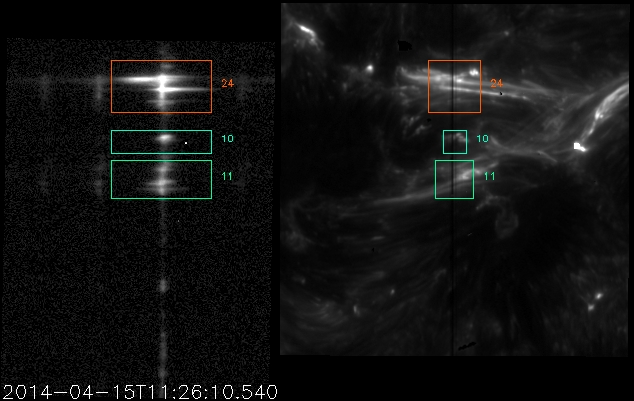
\includegraphics[scale=.4]{NESSF_img/01481.jpg}}
	\label{fig:eemovie}
\end{figure}

\begin{figure}
	\caption{Color map of event number 24. This RGB image is generated by binning line profile intensity around a typical sound speed, in this case $v = $ 60 km s$^{-1}$.  Blue is the total intensity  $\leq -v$, red is the total line intensity $\geq v$, and Green is the total intensity of the line core between $\pm v$. An example of this binning is illustrated in Figure \ref{fig:reconnect}.  A transition from a separated blue/red intensity to a broader green profile is similar to a progression proposed in Figure \ref{fig:reconnect}}
	\label{fig:eecolor}
	\centerline{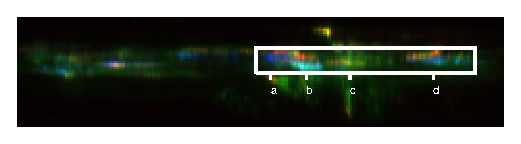
\includegraphics[scale=2]{NESSF_img/ee_color.eps}}
	
\end{figure}

The best tools currently available for studying magnetic reconnection in the lower solar atmosphere are high resolution spectrographs.  We propose a multi-instrument statistical study of small transient brightenings.  Our study will begin with a detailed statistical study of Si IV spectra taken by IRIS and transition to using Ne VII and O V images taken by MOSES and the EUV Slitless Imaging Spectrograph (ESIS)

	\subsection{Initial Survey and Event Selection}
	We began our study by building a large database of EEs.  To do this we selected a handful OBS IDs, IRIS observing programs, that best suited our needs.  These OBS are all sit-and-stare observations with $\leq 4$ second cadence, medium or better linelist, has limited spectral binning, and it must include the Si IV slit jaw data at least.   
	
	We opt to use sit-and-stare data, as opposed to slit rasters, for increased temporal resolution.  While it is easier to capture EEs using a rastered slit we have found that EEs evolve on a timescale much faster than the time it takes to complete even a small raster.  Therefore, the only way to capture EE dynamics fully is to sit and stare.  
	
	With EEs evolving on second time scales we must make a trade between image cadence and signal to noise ratio.  Over the last 4 years the FUV sensitivity of IRIS has diminished significantly.  An exposure length that was long enough in 2013 is not long enough now.  Fortunately for us EEs tend to be bright, allowing for good data with a sub four second exposure even with decreased sensitivity.  
	
	IRIS is an extremely flexible instrument that is limited in its data production by downlink telemetry bandwidth.  Two methods of reducing memory usage are truncating data in the spectral dimension and binning data at the CCD level.  We choose to use medium line list or better because it is the smallest line list that includes both Si IV spectral lines, $\lambda 1394$ \AA\  and $\lambda 1403$\AA.  We also allow more binning in spatial dimension, along the slit, than we do in the spectral dimension. If we hope to resolve narrow photospheric absorption lines, like Fe II and Ni II that only a pixel or two wide, we need to take advantage of IRIS' high spectral resolution.  We often bin spectra along the slit during analysis and therefore require less spatial resolution.
	
	Since the bulk of our analysis centers on Si IV spectra we require all OBS for this study to have at least the Si IV $\lambda1400$ \AA \ slit jaw images for context.  Slit jaw movies show what is going on around the slit and are very useful for identifying and sorting different event spatial structure.
	
	This criteria gave us 23 OBS from April 2014 to May 2017.  With more data coming down from IRIS everyday we will be able to expand this data set.  As we approach solar minima we will add more observations of quiet sun targets to look for any associated trends.  From these 23 OBS we have identified 581 events.  To do this we used an EE software package developed at Montana State University which provides a simple GUI for event selection as well as worked with an REU student during the summer of 2017 \citep{Bartz2018}.  An example of our software in action can be seen in Figure \ref{fig:eemap}.EE maps are made by integrating all material with a Doppler speed $\geq60$ km s$^{-1}$ and making an image with slit position on the vertical axis and time on the horizontal.  Then clumps of intensity in the image can be boxed via a click and drag interface.  Each box represents an event.
	
	An initial survey has shown our data set to cover a large portion of the solar disk, covering mostly active latitudes.  Most events last 20 min or less and cover less than 10'' of slit.
	
	Might want to pull in some figures of time/slit height scatter plots.

	
	\subsection{Spectral Diagnostic IRIS}
	Si IV has a peak formation temperature of $\approx 80,000$K placing it at the base of the transition region.  IRIS has revealed this line to be both optically thin during small flaring events and show a variety of optical depth effects \citep{Peter2014,Yan2015}.  Complex Si IV is line profiles are being used to draw new conclusions about the location EEs and the type of magnetic reconnection causing them.  We wish to study Si IV line profiles to determine which behaviors are statistically significant and which are anomalous events that contribute less to our overall understanding of EEs.
	
	We will start by sorting EEs into optically thin and optically thick events.  Si IV $\lambda 1394$ \AA \ and $\lambda 1403$ \AA \ lines maintain a 2:1 ratio during optically thin conditions  \citep{Mathioudakis1999}.  Deviations from this line ratio indicate an event has significant absorption or is optically thick.  Optically thick line profiles will need to be handled differently when determining Doppler shifts.  Absorption features would need to be masked off when analyzing line profiles.  
	
	%An example of how this could be handled is demonstrated by \citet{Peter2014}.
	The next step is to identify typical velocity distributions during EEs.  Observations of EEs in the past have shown them to be both bi-modal \citep{Innes1997,Rust2017} and have more continuous distributions with 3-D structure \citep{Fox2010,Innes2015,Rouppe2017}.  We will determine what portion of events deviate from the bi-modal Petschek reconnection picture of EEs by using Doppler maps like in Figure \ref{fig:eecolor}. By binning spectral intensity by Doppler shift we can quickly see events that have bi-directional flows (blue or red) and those that are more complicated and have significant line core emission (green).  Identifying blue/red to green transitions over time may help us understand the onset of the tearing mode instability and the transition to fast reconnection.
	
	The IRIS slit jaw movie give spatial context for each event.  Spatial context allows for further event classification. For example Figure \ref{fig:eemovie} shows a frame from the slit jaw movie associated with event 24 in Figure \ref{fig:eemap}.  From this frame we can see that event 24 is associated with a visible loop.  We can then correlate observed Doppler velocities with apparent motion along the loop.  An alternative could be a compact brightening with no obvious spatial structure, an observation off limb, a sun spot penumbra, etc.  This context is vital for interpreting spectral information.
	
	Say something about future work with C II or HMI?  Or is the scope getting too far out.
	

	

	\subsection{ESIS and MOSES-3}
	While IRIS provides high resolution spectral data in a few lines it fails in a few different areas.  Small field of view, a compromise between high cadence(sit-and-stare) and spatial resolution (rasters).  
	
	MOSES/ESIS proved the right lines for comparison, a larger FOV, and spectral data in a snapshot over the full field of view.  Talk about finishing up the developement of KSO and how you plan to tie in the data eventually.


\section{Scientific Impact}
%This section needs to answer the questions from the NASA strategic plan as well as quote language from the Decadal Survey. 5) Impact  This may also be the section to address the timely impact
%
%What causes the sun to vary?  How does the heliosphere respond?  What is the impact on Humanity?
Short and sweet.  Reconnection is a universal process that contributes tremendously to the variability of our sun and intern the Sun-Earth environment.

 
\section{Timeline}
Get a  degree, and maybe some extra money in the meantime.


\bibliography{NESSF18}


	

\end{document}


